\section{Challenges and design decisions}

With so many visualizations, finding a way to display them all in a meaningful way is quite challenging.
We opted for a one-page control panel displaying all our widgets, working best for Full-HD monitors (1920 by 1080 pixels or more).
Having a more responsive implementation would have cost us a lot of time, and would have been outside of the scope of this project.
We find that all components are closely linked together, and displaying them so eases the task of the user when they want to find insightful links out of visualizations.

The similarity graph got quite computationally heavy for later years -- there are more athletes and more runs to deal with.
To resolve this, we simply set a stricter threshold for similar skiers and eliminated all that were not connected to at least one other skier.
In-depth analysis -- see figure \ref{fig:threshold} -- has been made to choose the most interesting and the least demanding threshold.
There exists a fine balance between responsiveness and data shown.

\begin{figure}[ht]
    \centering
    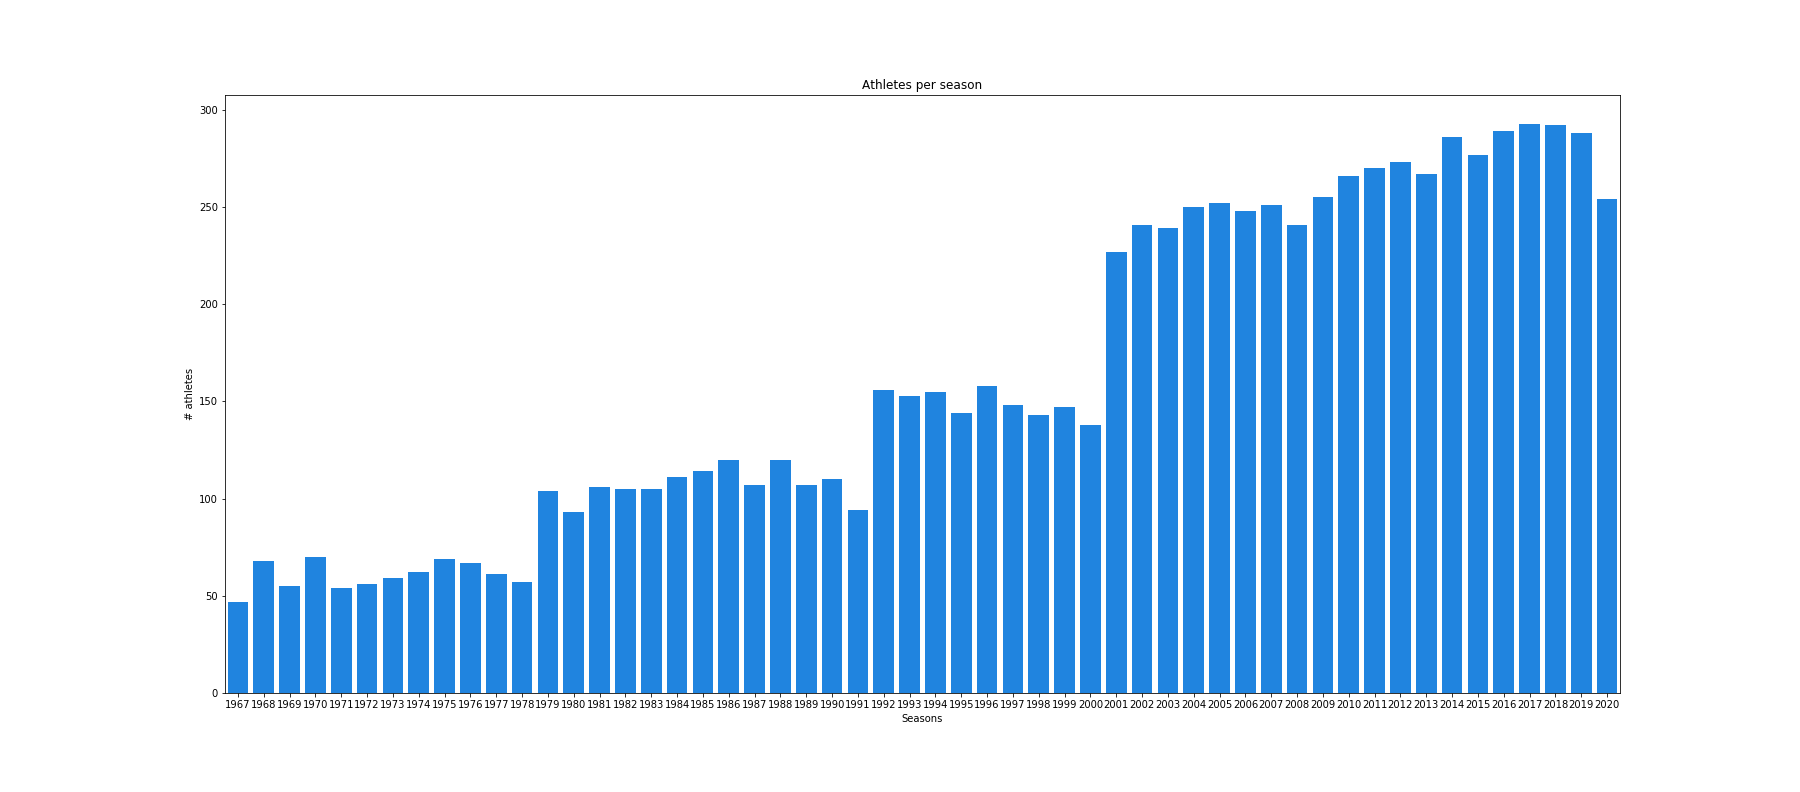
\includegraphics[width=\linewidth]{img/threshold.png}
    \caption{Analysis of the required thresholds for the similarity graph}
    \label{fig:threshold}
\end{figure}

Because of the way the FIS-website is designed, some skiers do not have a profile picture or personal information, although it is still stored on the website -- we simply missed them during scraping for diverse reasons.
We simply use a placeholder image for such cases.

We use Open Sans throughout our project, be it in this very process book, on the website, or in our screencast.
Colors of events have been harmonized throughout the whole project.
For example, a node of color in the similarity graph signifies that the skier has won a World Cup ranking during the season.
We use external images for the skier profiles, so we had to make sure that they had the correct size when they appear in our visualizations.

The website is based on a grid layout, built with Bootstrap.
This tool allowed us to quickly merge and harmonize all of our work.
It provides useful user interface (UI) components for a uniform style, based on the best practices of the web.
We also used it to code the modal of the profile statistics.
As a technical detail, we only used one \texttt{iframe}, to display the screencast directly from YouTube.

All of the data displayed on our website is precomputed and present in their own json files.
This is of course for performance reasons, as otherwise the site would take ages to load each time we switch the season or the gender.
This increases the amount of transferred data, but only files used for the current visualization are loaded.
Thanks to the browser's cache, the user can easily reload the same visualizations and still have that data locally.

We use the following libraries, imported via content delivery networks (CDN), in our project:

\begin{itemize}
    \item \texttt{d3.js} for the graphs
    \item \texttt{Bootstrap} for the style and layout
    \item \texttt{Popper}, as a dependency of bootstrap
    \item \texttt{ion.rangeslider} for the two sliders (which has a slight bug in the tick alignment unfortunately)
    \item \texttt{Leaflet} for the map
    \item \texttt{JQuery} for the DOM manipulation
\end{itemize}
